%%%%%%%%%%%%%%%%%%%%%%%%%%%%%%%%%%%%%%%%%%%%%%%%%%%%%%%%%%%%%%%%%%%%%%%%%%%%%%%%
\chapter{Оценка качества реализованного способа извлечения ВОП}
\label{chap:quality}
%%%%%%%%%%%%%%%%%%%%%%%%%%%%%%%%%%%%%%%%%%%%%%%%%%%%%%%%%%%%%%%%%%%%%%%%%%%%%%%%

В данном разделе проводится оценка качества разработанной технологии извлечения ВОП. Качество оценивается путем изучения влияния эвристик предобработки и параметров на выбраные метрики качетсва, а также путем экспертной оценки.

\section{Определение доли найденных ВОП}

На рисунке~\ref{fig:tickets_distr} изображена помесячная гистограмма результатов, показывающая соотношение количества исходных обращений, предобработанных и отфильтрованных обращений, а также найденных ВОП. 

\begin{figure}[tph!]
\centerline{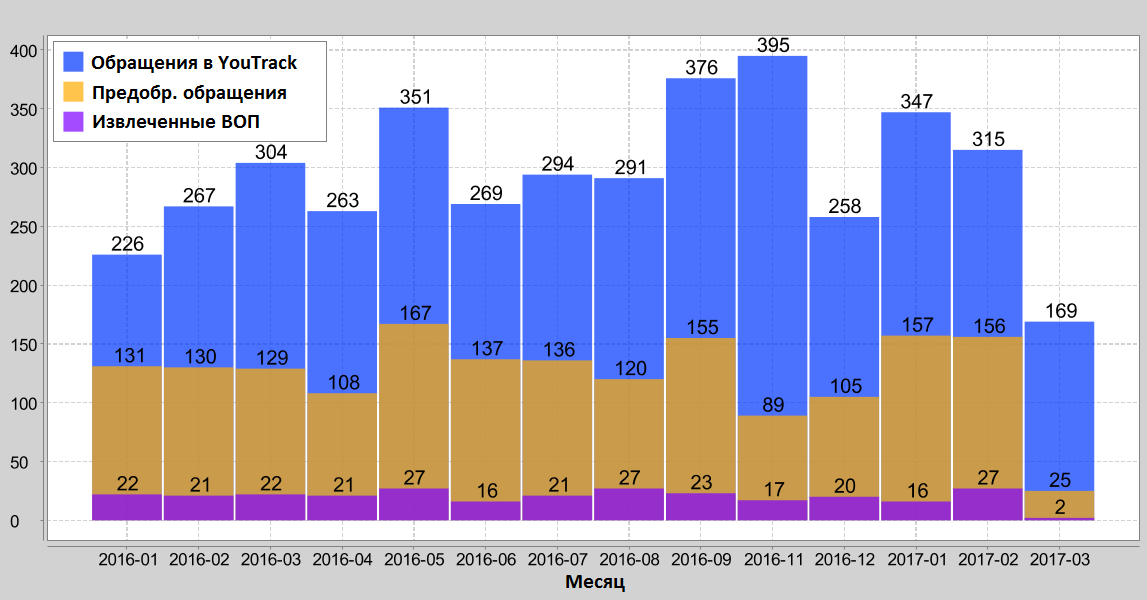
\includegraphics[width=11.5cm]{fig/tickets_distr.png}}
    \caption{Гистограмма извлеченных ВОП}
    \label{fig:tickets_distr}
\end{figure}

По графику видно, что медианное значение количества вопросов, на которое может быть расширен раздел с ЧЗВ, составляет 21 вопрос в месяц. В среднем доля ВОП составляет 6,8\%.

Как упоминалось ранее, анализируемые данные не являются предварительно размеченными, в связи с чем, отсутвует возможность посчитать полноту и точность решения. Воспользуемся дургими способами оценки качества найденных ВОП, которые рассмотрены далее.

\section{Оценка влияния эвристик и параметров на качество ВОП}

Для оценки качества алгоритма использовались следующие метрики: косинус между вопросом и темой, косинус между ответом и темой. Таблица~\ref{quality} показывает влияние этапов предобработки и параметров алгоритма на значения метрик. Характеристики анализируемых данных включают: 6500 обращений, 19700 комментариев, более 45000 различных слов.

В работе~\cite{original} было установлено, что ВОП, признанные экспертами подходящими для публикации в ЧЗВ, имеют более высокие значения косинусного расстояния (\cite{original},~секция~VI--C). В таблице~\ref{quality} видно, что применение эвристик предобработки и фильтров (за исключением фильтра тем) положительно влияет на косинус вопросов и ответов. Изменение параметров в большую сторону позволяет находить меньшее количество более качественных, с точки зрения косинусного расстояния, ВОП.

\section{Экспертная оценка}

Экспертная оценка проводилась только для оптимального набора параметров. В качестве эксперта выступил разработчик YouTrack, которому было предложено 20 ВОП с наибольшим значением гармонического среднего. Эксперту необходимо было оценить, какие из предложенных ВОП подходят для публикации в ЧЗВ. Результаты представлены в таблице \ref{qualityExpert}. Доля подходящих для публикации ВОП составила 50\%, для \cite{original} данный показатель составил 37\%. 

Да момент написания статьи работа еще не была завершена, планируется дополнительная оптимизация с целью повышения доли подходящих для публикации ВОП и получение дополнительных экспертных оценок. 

\begin{landscape}
\begin{table*}[t]
  \caption{Влияние эвристик и параметров на медианные значения метрик}
  \label{quality}
  \centering
  \begin{tabular}{|c|c|c||c|c|c|c|}
     \hline
      \parbox[t]{3cm}{\textbf{Исследуемый параметр}} &%
     \parbox[t]{2cm}{\textbf{Старое значение}} &%
     \parbox[t]{1.7cm}{\textbf{Новое значение}} &%
     \textbf{Перплексия} &%
     \parbox[t]{2cm}{\textbf{Количество ВОП}} &%
     \textbf{$\cos(Q,T)$} &%
     \textbf{$\cos(A,T)$} \\
	 \hline
     \parbox[t]{3cm}{Оптимальные\\параметры} &%
     - &%
     - &%
	 1864 &%
     357 &%
 	 0.396 &%
     0.413 \\
  	 \hline
     \parbox[t]{3cm}{Эвристики отображения (\ref{subsec:lnfheur})} &%
     вкл &%
     выкл &%
	 1971 &%
     361 &%
 	 0.371 &%
     0.395 \\
	 \hline
	 \parbox[t]{3cm}{Эвристики тем.\\модел. (\ref{subsec:ldaheur})} &%
     вкл &%
     выкл &%
	 2016 &%
     384 &%
 	 0.369 &%
     0.391 \\
	 \hline
\parbox[t]{3cm}{Фильтр\\обращений (\ref{subsec:ticketfilter})} &%
     вкл &%
     выкл &%
	 1924 &%
     403 &%
 	 0.370 &%
     0.388 \\
	 \hline
\parbox[t]{3cm}{Фильтр тем (\ref{subsec:topicfilter})} &%
     вкл &%
     выкл &%
	 1791 &%
     472 &%
 	 0.393 &%
     0.416 \\
     \hline
\parbox[t]{3cm}{Порог выбора\\темы LDA (\ref{subsec:lda})} &%
     0.25 &%
     0.0 &%
	 1853 &%
     376 &%
 	 0.366 &%
     0.404 \\
     \hline
\parbox[t]{3cm}{Порог выбора\\темы LDA (\ref{subsec:lda})} &%
     0.25 &%
     0.4 &%
	 1871 &%
     302 &%
 	 0.399 &%
     0.421 \\
     \hline
\parbox[t]{3cm}{Мин. значение\\косинуса (\ref{subsec:findqa})} &%
     0.15 &%
     0.0 &%
	 1860 &%
     394 &%
 	 0.337 &%
     0.359 \\
     \hline
\parbox[t]{3cm}{Мин. значение\\косинуса (\ref{subsec:findqa})} &%
     0.15 &%
     0.3 &%
	 1864 &%
     288 &%
 	 0.387 &%
     0.419 \\
     \hline         
\parbox[t]{3cm}{Мин. доля\\ВОП (\ref{subsec:deleteunfocusedtopics})} &%
     0.1 &%
     0.0 &%
	 1869 &%
     376 &%
 	 0.384 &%
     0.407 \\
     \hline
\parbox[t]{3cm}{Мин. доля\\ВОП (\ref{subsec:deleteunfocusedtopics})} &%
     0.1 &%
     0.2 &%
	 1850 &%
     324 &%
 	 0.391 &%
     0.417 \\
     \hline     
  \end{tabular}

\end{table*}
\end{landscape}

\begin{table}[!ht]
\caption{Экспертная оценка}
\label{qualityExpert}
\centering
\begin{tabular}{|c|c|c|}
\hline
Категория ВОП & Количество & Доля, \% \\
\hline
\parbox[t]{4cm}{\textbf{Общее количество}} & 358 & 100 \\

	 \hline
\parbox[t]{4cm}{Подходит для публикации без редактирования} & 262 & 73 \\

	 \hline
\parbox[t]{4cm}{Подходит для публикации с редактированием вопроса или ответа} & 17 & 5\\

	 \hline
\parbox[t]{4cm}{Не подходит для публикации. Некорректный вопрос} & 17 & 5\\

	 \hline
\parbox[t]{4cm}{Не подходит для публикации. Некорректный ответ} & 62 & 17\\
\hline
\end{tabular}
\end{table}


\section{Резюме}